\section{Background}
Dynamic cell-cell interactions coordinate bidirectional information transfer in the immune system and control the potency and the scope of effector responses \cite{Batista2013}. One of the most important of these interactions is the immunological synapse (IS) formed between a cytotoxic T lymphocyte (CTL) and the infected or transformed target cell it aims to destroy \cite{Dustin2010, Stinchcombe2007}. IS formation is rapidly induced by recognition of cognate peptide–major histocompatibility complex (MHC) on the target cell by T cell antigen receptors (TCRs) on the CTL. Once firm contact is established, the CTL secretes a toxic mixture of granzyme proteases and the hydrophobic protein perforin into the intercellular space. Perforin forms pores in the target cell membrane that stimulate the uptake of granzymes into the cytoplasm, where they induce apoptosis by cleaving specific substrates \cite{Thiery2014}. Perforin- and granzyme- mediated killing is the most prevalent mode of lymphocyte cytotoxicity, and it likely plays an important role in cellular immunotherapy approaches against cancer \cite{Martinez-Lostao2015}.

IS formation is accompanied by dramatic reorganization of both microtubules and filamentous actin (F-actin) \cite{Liu2015}. Within minutes of TCR stimulation, the centrosome (also called the microtubule-organizing center) moves to a position just beneath the IS. The centrosome is closely associated with lytic granules, the secretory lysosomes that store perforin and granzyme, and its reorientation positions these granules next to the synaptic membrane \cite{Stinchcombe2007}. This promotes the directional secretion of granule contents into the intercellular space, enhancing both the potency and the specificity of killing. Whether (and how) F-actin remodeling contributes to cytotoxicity is, by comparison, less clear. Our current conception of synaptic F-actin is strongly influenced by imaging studies in which the target cell is replaced by a glass surface or a supported bilayer containing stimulatory TCR ligands. In this context, T cells form radially symmetric synapses characterized by intense F-actin accumulation at the periphery and depletion from the center \cite{Bunnell2001, LeFloch2013, Kaizuka2007, Yi2012}. This annular configuration is thought to encourage lytic granule fusion at the center of the IS by clearing F-actin from the plasma membrane in this zone \cite{Stinchcombe2007, Stinchcombe2006, Ritter2015}. Although this model is conceptually appealing, it is unclear how well it applies to granule release in bona fide CTL–target cell conjugates, where synaptic F-actin rings are less apparent and, when observed, often quite transient. Synaptic F-actin is also highly dynamic, forming protrusions and lamellipodial sheets that exhibit both centripetal retrograde flow and radial anterograde movement \cite{Yi2012, Ritter2015, Sage2012, Cai2017, Nguyen2008}. These dynamics enable T cells to impart mechanical force across the IS \cite{Husson2011, Bashour2014}. In CTLs, the capacity to exert synaptic force is notably correlated with cytotoxic potential \cite{Basu2016}. Biophysical and imaging experiments suggest that force enhances cytotoxicity by increasing the membrane tension of the target cell, which in turn promotes the pore-forming activity of secreted perforin. Here, we applied microfabrication and high-resolution live imaging to investigate how CTLs mechanically potentiate the chemical activity of perforin, a process we refer to as mechanopotentiation. Using stimulatory micropillar arrays that trigger IS formation in three dimensions, we have found that lytic granule release occurs at the base of F-actin–rich synaptic protrusions that extend into the antigen-presenting surface. These protrusions, which are generated by the Wiskott-Aldrich syndrome protein (WASP) and the actin related protein (Arp)2/3 actin nucleation complex, are required for synaptic force exertion and cytotoxic efficiency. Our results provide insight into how cytotoxic lymphocytes organize mechanical output and demonstrate how three-dimensional architecture influences the functionality of communicative interfaces in the immune system.

\subsection{Force exertion through the actin cytoskeleton}
The actin cytoskeleton is a dynamic network of actin polymers and associated actin binding proteins. It is the primary means by which the T cell achieves its shape, and its migratory and interactive capabilities against the target cell. Central actin depletion is reported as necessary for granule fusion at the immune synapse, a reminder of the intimate link between the actin cytoskeletal dynamics and the killing functions of the T cell. Accordingly, the T cell uses actin-mediated mechanical force against the target cell in order to achieve its full cytotoxicity (see section \ref{Modifying target cell sensitivity to perforin}) \cite{Basu2016}. Perturbations of PTEN (an antagonist of PI3K-dependent F-actin remodeling via Dock2, see section \ref{The immunological synapse and the T cell cytoskeleton}) enhanced synapse formation, strongly increased force exertion, and markedly increased killing \cite{LeFloch2013, Basu2016}. This perturbation did not affect granule organization or release, suggesting that actin-mediated force is at least partially responsible for this increased cytotoxic effect \cite{Basu2016}. The T cell has also been reported to form protrusions of varying function - some groups highlight the ability of these protrusions to facilitate antigen recognition \cite{Sage2012}, enriched T cell activation \cite{Pettmann2018}, and trogocytosis \cite{Kim2018}. In totality, these findings highlight an intimate link between proper IS formation and optimal cytotoxicity that is mechanical in nature.

\subsection{Modifying target cell sensitivity to perforin}
\label{Modifying target cell sensitivity to perforin}
The insertion of perforin into the target cell membrane requires overcoming an energetic barrier that is imposed by the features of the plasma membrane, namely the hydrophobic inner leaflet and the tensile state of the target cell surface. Membrane tension is a measure of the cost of increasing the membrane area, as opposed to cortical tension \cite{Sitarska2020}. Although intimately related to membrane tension (see Figure \ref{fig:membranecorticaltension}), cortical tension is strictly defined the tensile forces involved in cytoskeletal cortex \cite{Sitarska2020}. Membrane tension can be affected in many ways, particularly in cell surfaces as compared to pure lipid vesicles, because of the following factors: the presence of transmembrane proteins, membrane-cytoskeletal interactions within the cell itself, and potential external forces imparted by interacting cells \cite{Sitarska2020}. 

\begin{figure}[htbp]
	\centering
	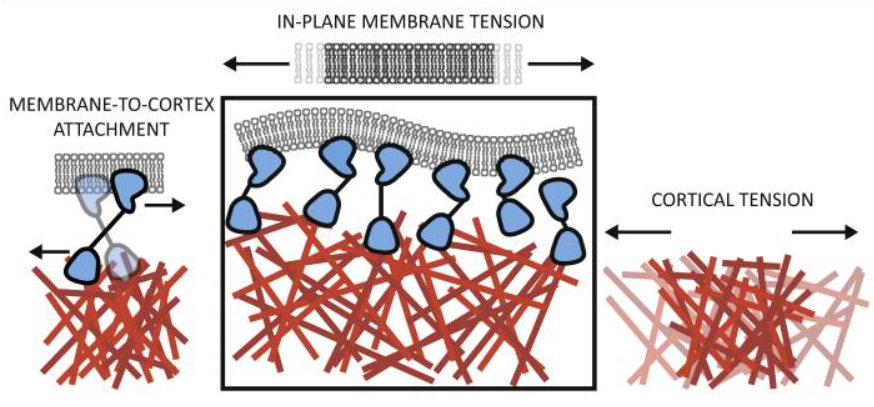
\includegraphics[width=0.9\textwidth]{../figures/chapter2/membranecorticaltension.png}
	\caption{Mechanics of the plasma membrane and the underlying actomyosin cortex.}
	\caption*{Both the plasma membrane (gray) and the cortex (red) are under tension, a measure of the energetic cost of increasing their area. In cells, membrane tension arises from both in-plane tension (final distance between lipids exaggerated for clarity) and membrane-to-cortex-attachment (MCA, blue), which is related to cortical tension (right). This figure is adapted from \cite{Sitarska2020}.}
	\label{fig:membranecorticaltension}
\end{figure}

\begin{figure}[htbp]
	\centering
	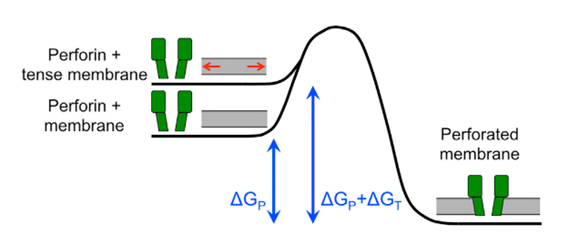
\includegraphics[width=\textwidth]{../figures/chapter2/reactioncoordinate.png}
	\caption{Perforin entry into target cell membrane reaction coordinate.}
	\caption*{Schematic diagram of the reaction coordinate for perforin pore formation in a membrane, illustrating how increased membrane tension can effectively reduce the activation barrier of the process. $\Delta$GP = free energy of pore formation, $\Delta$GT = free energy of tension release. This figure is adapted from \cite{Basu2016}.}
	\label{fig:reactioncoordinate}
\end{figure}

T cells manipulate the membrane tension of target cells in order to sensitize the target cell to perforin \cite{Basu2016}. Therefore, it follows that increased membrane tension has been found to be a contributing factor in overcoming the energy barrier imposed by the plasma membrane (Figure \ref{fig:reactioncoordinate}), effectively sensitizing the target cell to perforin. Tumor cells grown on stiffer hydrogels (resulting in higher levels of membrane stiffness as indicated by morphology) were more sensitive to recombinant perforin lysis in a T cell-free system, indicating that the manipulation of target cell membrane tension is one avenue by which T cells may potentiate their killing function \cite{Basu2016}. T cells modified to exert more physical force displayed higher levels of killing, despite similar levels of degranulation as compared to control cells \cite{Basu2016}. However, the nature of the exact cellular structures that T cells formed in order to physically manipulate the target and what molecular pathways may regulate them remained unknown, and was the primary interest of the study detailed in this chapter.


\section{Results} 

\subsection{CTLs form actin-rich protrusions on stimulatory micropillars}
Synaptic force exertion can be measured by imaging T cells on arrays of flexible polydimethylsiloxane (PDMS) micropillars bearing immobilized TCR ligands and adhesion proteins (Figure \ref{fig:fig1pillarscartoon}) \cite{Bashour2014, Basu2016}. T cells form IS-like contacts with these arrays and induce pillar deflections that can be converted into force vectors based on the known dimensions and composition of the pillars. Using this approach, we previously found that lytic granule release tends to occur in regions of active pillar deflection \cite{Basu2016}. This result raised the possibility that there might be specific structures within the IS that mechanopotentiate perforin function by imparting force in close proximity to granule secretion.

\begin{figure}[htbp]
	\centering
	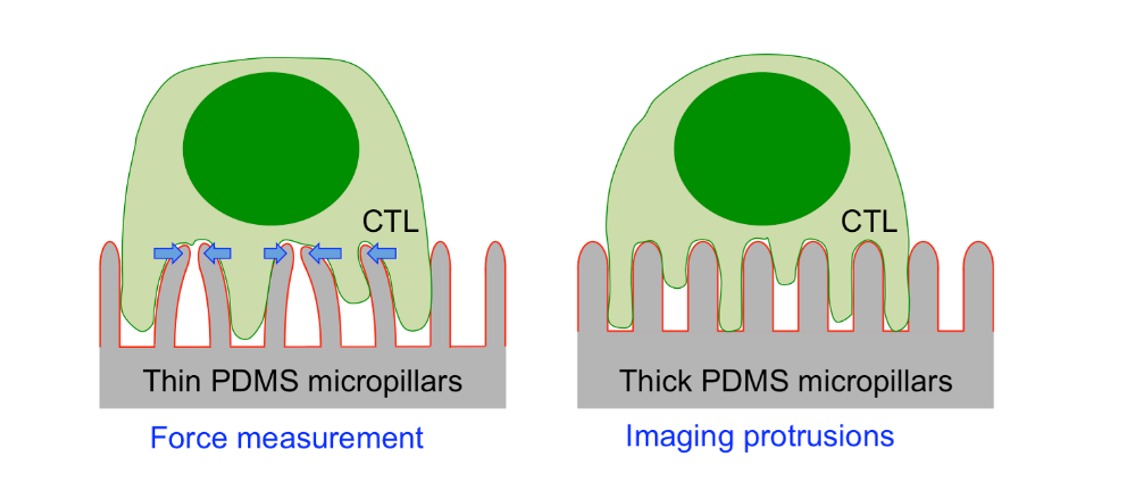
\includegraphics[width=\textwidth]{../figures/chapter2/fig1pillarscartoon.png}
	\caption{Using PDMS micropillars as 3D environment to observe and measure CTL cytoskeletal structures.}
	\caption*{Schematic diagram of thin micropillars used for force measurements (left) and thicker micropillars used for imaging protrusions (right).}
	\label{fig:fig1pillarscartoon}
\end{figure}

To identify candidate structures that could be involved in this mechanopotentiation, we closely examined the dynamic architecture of CTL synapses on micropillar arrays. For these experiments, we used primary CTLs expressing the OT1 TCR, which is specific for the ovalbumin 257–264 peptide presented by the class I MHC protein H2-$K^{b}$ [H2-$K^{b}$–ovalbumin (OVA)]. OT1 CTLs were retrovirally transduced with Lifeact–green fluorescent protein (GFP), a fluorescent probe for F-actin, and imaged by confocal microscopy on micropillars coated with H2-Kb-OVA and ICAM1 (intercellular adhesion molecule 1), a ligand for the $\alpha$L$\beta$2 integrin LFA1. The pillars in these arrays (1 to 1.5 $\mu$m in diameter and 4 to 5 $\mu$m tall) were thicker, shorter, and therefore more rigid than the pillars used for T cell force measurements (0.7 $\mu$m in diameter and 6 $\mu$m tall) (Figure \ref{fig:fig1pillarscartoon}). These thicker pillars are not substantially deflected by CTLs and function as a regularly crenulated stimulatory surface that facilitates quantitative assessment of IS growth in three dimensions.

Within minutes of initial contact with the arrays, the CTLs formed F-actin–rich protrusions that invaded the spaces between adjacent pillars (Figure \ref{fig:fig1pillars}a). Time-lapse experiments using both confocal and lattice light-sheet microscopy revealed that the F-actin in these protrusions was highly dynamic, coruscating up and down the length of each pillar (Figure \ref{fig:fig1pillarscartoon}a). Periodically, F-actin–free gaps appeared at the base of the protrusions, in the regions around the pillar tops. During protrusion growth, F-actin accumulation was often strongest at the leading edge, implying a causative relationship between actin polymerization and the formation of these structures (Figure \ref{fig:fig1actinleadingedge}b). Most of the microtubule cytoskeleton, by contrast, was constrained to the region above the pillars, although individual microtubules were observed to extend into a subset of protrusions (Figure \ref{fig:fig1pillars}b). In most cells, the centrosome reoriented to a position in the plane of the pillar tops but did not proceed into the interpillar spaces. Hence, on micropillar arrays, CTLs form dynamic, F-actin–rich protrusions at the IS that exclude the centrosome.

\begin{figure}[htbp]
	\centering
	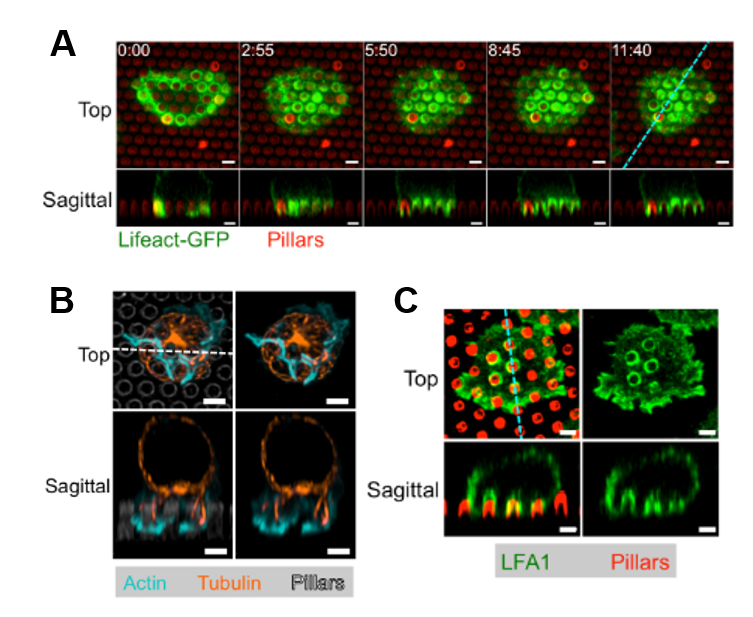
\includegraphics[width=\textwidth]{../figures/chapter2/fig1pillars.png}
	\caption{Characterizing the architecture of protrusions using micropillars.}
	\caption*{\textbf{(A-C)}: OT1 CTLs were imaged by confocal microscopy on micropillars bearing H2-$K^{b}$-OVA and ICAM1. z-projection images (top views) are shown above with sagittal views below. Dashed lines [cyan in \textbf{(A)} and \textbf{(C)}; white in \textbf{(B)}] denote the slicing plane used for the sagittal images. \textbf{(A)}: Time-lapse montage of a representative CTL expressing Lifeact-GFP, with micropillars shown in red. \textbf{(B)}: Fixed image of a representative CTL stained with phalloidin (to visualize F-actin) and antitubulin antibodies. Micropillars are shown in gray in the left images. \textbf{(C)}: Fixed image of a representative CTL stained with anti-LFA1 antibodies, with micropillars shown in red. All scale bars, 2 $\mu$m. Mitchell Wang, Fella Tamzalit, and Morgan Huse performed these experiments.}
	\label{fig:fig1pillars}
\end{figure}

\begin{figure}[htbp]
	\centering
	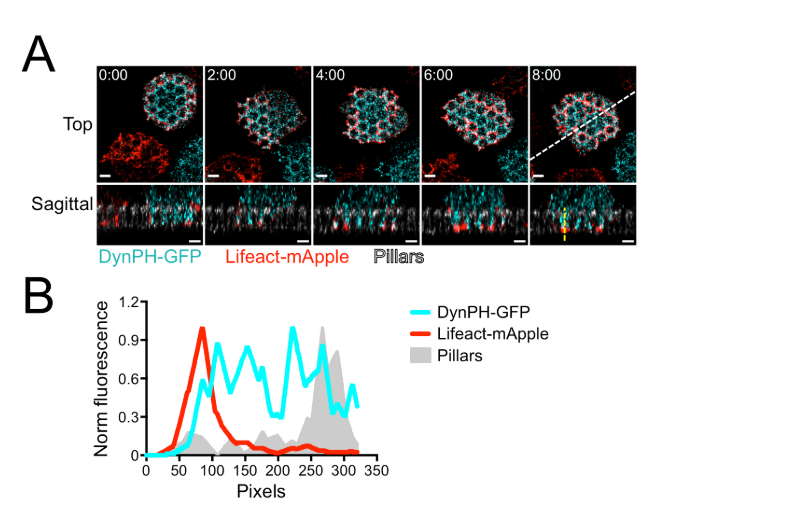
\includegraphics[width=\textwidth]{../figures/chapter2/fig1actinleadingedge.png}
	\caption{F-actin accumulates at the leading edges of synaptic protrusions.}
	\caption*{OT1 CTLs expressing Lifeact-mApple and DynPH-GFP (a membrane marker) were imaged by confocal microscopy on fluorescent micropillars bearing H2-Kb-OVA and ICAM1. \textbf{(A)}: Time-lapse montage of a representative CTL, with z-projection images (top views) shown above and sagittal views below. The white dashed line denotes the slicing plane used for the sagittal images. Pillars (gray) appear in the sagittal images only. Time in M:SS is indicated in the upper left corner of each top view. Scale bars = 2 $\mu$m. \textbf{(B)}: Linescan (derived from the dashed yellow line in \textbf{(A)}) showing normalized fluorescence intensity of DynPH-GFP, Lifeact-mApple, and the pillars. Mitchell Wang, Fella Tamzalit, and Morgan Huse performed these experiments.}
	\label{fig:fig1actinleadingedge}
\end{figure}

During initial cell spreading, invasion into the micropillar zone was typically constrained to the periphery of the contact (Figure \ref{fig:fig1pillars}a). However, once the radial size of the IS stabilized, after around 60s, protrusions formed in the more central regions of the interface. This was intriguing to us because previous studies had indicated that lytic granules accumulate beneath the more central IS domains \cite{Stinchcombe2007, Stinchcombe2006, Beal2009, Stinchcombe2001}. To investigate the spatial relationship between synaptic protrusions and lytic granules, we imaged CTLs expressing Lifeact-mApple together with a GFP-labeled form of the lysosomal-associated membrane protein 1 (Lamp1-GFP). Lytic granules appeared as a cluster of distinct compartments within the CTL cytoplasm. In the first 2 min of contact formation, the granule cluster moved downward, settling around 5 $\mu$m from the cell front, roughly at the level of the pillar tops (Figure \ref{fig:fig1granulecentralization}). This behavior implied a close association between granules and the centrosome, as previously reported \cite{Stinchcombe2006, Kupfer1984, Stinchcombe2001}.

\begin{figure}[htbp]
	\centering
	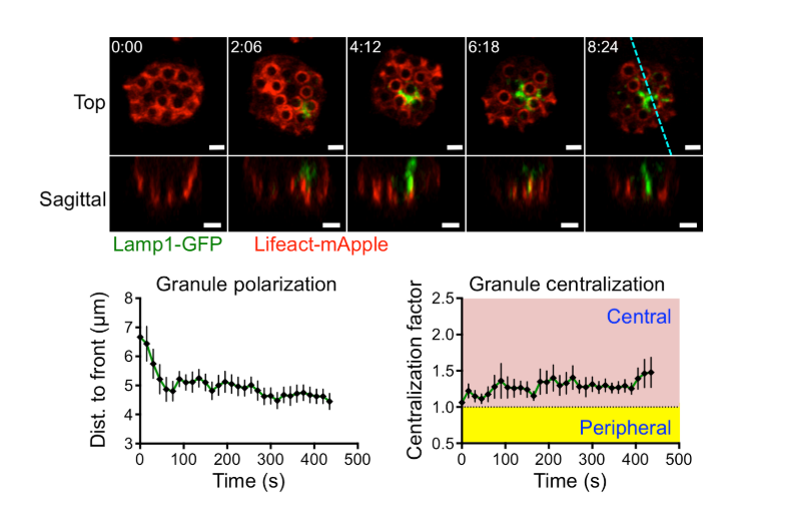
\includegraphics[width=\textwidth]{../figures/chapter2/fig1granulecentralization.png}
	\caption{Granules polarize towards the center of the immune synapse.}
	\caption*{Above, time-lapse montage of a representative CTL expressing Lifeact-mApple and Lamp1- GFP. Below left, mean distance between the lytic granule cloud and the cell front, graphed against time. Below right, centralization factor analysis of Lamp1-GFP. In both graphs, time 0 denotes initial contact with the pillars and error bars indicate SEM. n = 10. Mitchell Wang, Fella Tamzalit, and Morgan Huse performed these experiments.}
	\label{fig:fig1granulecentralization}
\end{figure}

After orienting downward, the granules tended to occupy central locations within the IS, which we quantified by calculating the normalized proximity of granule fluorescence to the IS center of gravity (COG) (Figure \ref{fig:fig1centralizationfactor}). Analysis of this “centralization factor” revealed that the granules tended to be closer to the center of the IS than would be expected by chance (Figure \ref{fig:fig1granulecentralization}).

\begin{figure}[htbp]
	\centering
	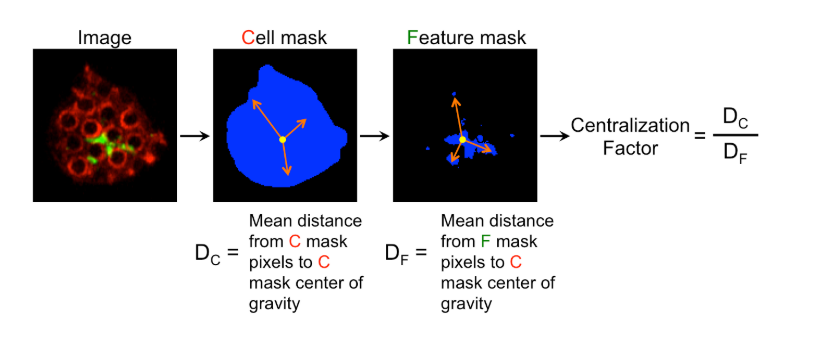
\includegraphics[width=\textwidth]{../figures/chapter2/fig1centralizationfactor.png}
	\caption{Centralization factor analysis.}
	\caption*{The centralization factor compares the mean distance between a given feature within the IS (e.g. lytic granules) and the IS center of gravity ($D_F$) to the mean distance between all positions within the IS and the IS center of gravity ($D_C$). Mitchell Wang, Fella Tamzalit, and Morgan Huse performed these experiments.}
	\label{fig:fig1centralizationfactor}
\end{figure}

The proximity of lytic granules to the base of synaptic protrusions at the center of the IS raised the possibility that these structures might be involved in cytolytic mechanopotentiation. Synaptic protrusions were highly enriched in LFA1 (Figure \ref{fig:fig1pillars}c), consistent with them being strongly adhesive and capable of exerting force. Previously, we found that mechanopotentiation requires phosphoinositide 3-kinase (PI3K) signaling and is enhanced by the depletion of phosphatase and tensin homolog (PTEN) that antagonized PI3K. Short hairpin RNA (shRNA)-mediated suppression of PTEN augmented F-actin accumulation in synaptic protrusions (Figure \ref{fig:fig1ptenprotrusions}b and c), further supporting the idea that these structures transmit forces that promote cytotoxicity.

\begin{figure}[htbp]
	\centering
	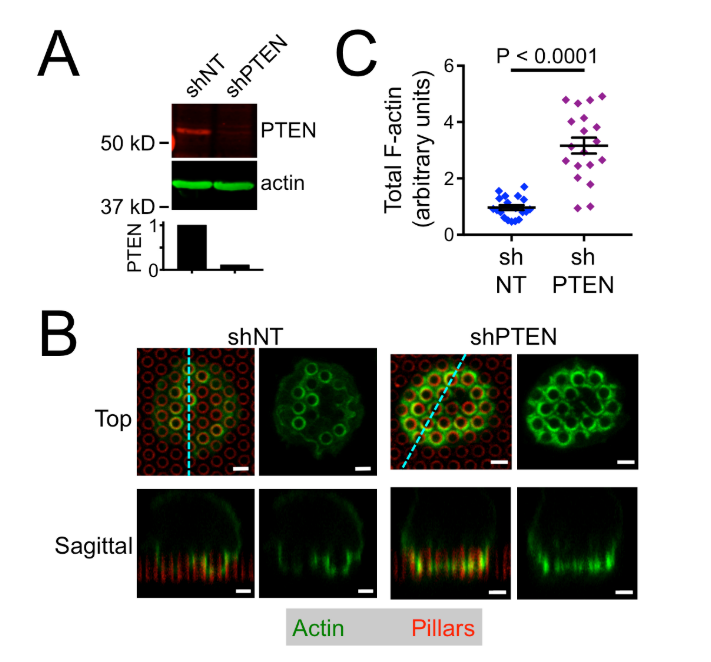
\includegraphics[width=\textwidth]{../figures/chapter2/fig1ptenprotrusions.png}
	\caption{PTEN depletion enhances F-actin accumulation in protrusions.}
	\caption*{OT1 CTLs expressing shRNA against PTEN (shPTEN) or a control nontargeting shRNA (shNT) were applied to fluorescent micropillars bearing H2-$K^{b}$-OVA and ICAM1, fixed, and stained with phalloidin. \textbf{(A)}: Immunoblot analysis of PTEN expression in shNT and shPTEN CTLs. Actin served as a loading control. Bars denote intensity of PTEN bands. \textbf{(B)}: Representative images of shNT and shPTEN CTLs, with z-projection images (top views) shown above and sagittal views below. Cyan dashed lines denote the slicing planes used for the sagittal images. Scale bars = 2 $\mu$m. \textbf{(C)}: Quantification of sum F-actin intensity on micropillar arrays. Error bars denote SEM. N = 19 for each cell type. P calculated from two-tailed Student’s T-test. Fella Tamzalit and Morgan Huse performed these experiments.}
	\label{fig:fig1ptenprotrusions}
\end{figure}

\subsection{Granule fusion occurs at the base of synaptic protrusions}
Granule fusion events can be detected in single-cell imaging experiments with a fluorescent reporter containing a pH-sensitive GFP (pHluorin) fused to the granule-targeting domain of Lamp-1 \cite{Friedman2020}. Within lytic granules, the low pH environment quenches the fluorescence of pHluorin-Lamp1. Granule fusion with the plasma membrane, however, neutralizes the pH around the reporter, leading to a rapid increase in fluorescence. To explore the relationship between cytolytic secretion and synaptic protrusions, we imaged OT1 CTLs expressing pHluorin-Lamp1 by confocal and lattice  light-sheet microscopy on fluorescent micropillars coated with H2-$K^{b}$-OVA and ICAM1I (Figure \ref{fig:fig2degranulation}). Protrusions were visualized in these experiments either via Lifeact-mRuby2 or by staining with a fluorescent Fab against the surface marker CD45. After IS formation, fusion events appeared as sudden flashes of GFP fluorescence, which were often visible for only one time point. These events clustered close to the plane of the pillar tops (Figure \ref{fig:fig2degranulation}a, b, c and e), the same vertical zone occupied by lytic granules and the centrosome. This position was well behind the leading edge of CTL protrusions, which extended about 5 $\mu$m into the interpillar space.

\begin{figure}[htbp]
	\centering
	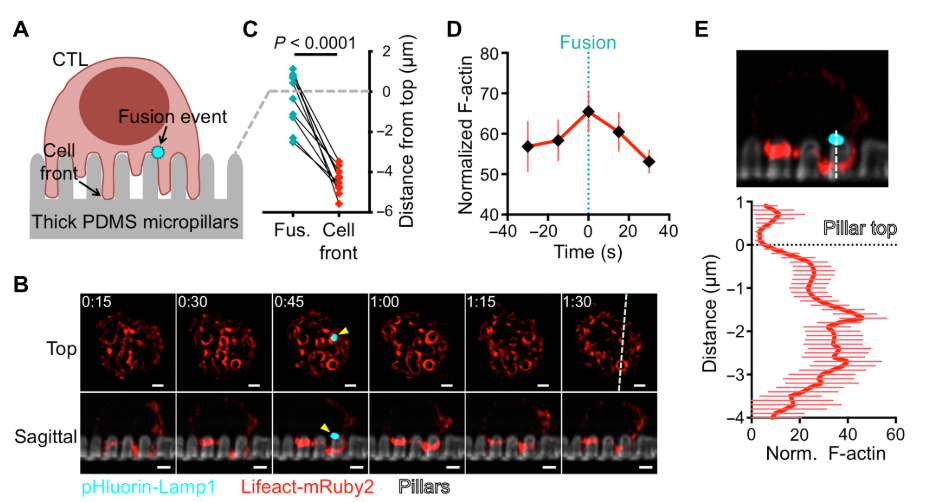
\includegraphics[width=\textwidth]{../figures/chapter2/fig2degranulation.png}
	\caption{Granule fusion occurs at the base of synaptic protrusions.}
	\caption*{\textbf{(A)}: Schematic diagram showing lytic granule fusion (visualized by pHluorin-Lamp1) on micropillar arrays. \textbf{(B to E)}: OT1 CTLs expressing pHluorin-Lamp1 were imaged by confocal \textbf{(C)} or lattice light-sheet \textbf{(B, D, and E)} microscopy on micropillars bearing H2-$K^{b}$-OVA and ICAM1. \textbf{(B)}: Time-lapse montage of a representative CTL expressing Lifeact-mRuby2 and pHluorin-Lamp1, with micropillars shown in gray. z-projection images (top views) are shown above with sagittal views below. The white dashed line denotes the slicing plane used for the sagittal images. Yellow arrowheads indicate the fusion event. Time in minutes:seconds is indicated in the upper left corner of each top-view image. Scale bars, 2 $\mu$m. \textbf{(C)}: Graph showing the vertical displacements of fusion events (Fus., cyan) relative to the plane of the pillar tops (dashed gray line) along with the corresponding position of the cell front (red, visualized with a fluorescent Fab fragment against CD45). n = 11 events. P values were calculated from two-tailed paired Student’s t test. \textbf{(D)}: F-actin accumulation in the region of granule fusion in z-projection images of CTLs expressing Lifeact-mRuby2 and pHluorin-Lamp1. Graph shows the average Lifeact-mRuby2 intensity within a 1-$\mu$m-diameter circle centered on the fusion site, starting two time points before the fusion event and ending two time points after. \textbf{(E)}: Below, mean normalized (Norm.) Lifeact-mRuby2 intensity derived from linescans vertically bisecting the midpoint of the granule fusion site. The dotted black line denotes the plane of the pillar tops. Above, a representative image used for the analysis, with the linescan region indicated by the dashed white line. Error bars in \textbf{(D)} and \textbf{(E)} denote SEM. n = 18 events. Mitchell Wang, Fella Tamzalit, and Morgan Huse performed these experiments.}
	\label{fig:fig2degranulation}
\end{figure}

Granule fusion was not observed in zones of sustained F-actin depletion. Instead, it tended to occur in regions containing synaptic protrusions (Figure \ref{fig:fig2degranulation}a). To quantify this effect, we determined the Lifeact-mRuby2 intensity over time in the 1-$\mu$m-diameter synaptic domain around each fusion site. F-actin accumulation within this domain actually increased modestly during granule fusion (Figure \ref{fig:fig2degranulation}d), implying that cytolytic secretion and protrusion growth could occur concurrently in the same region. Linescans of sagittal slice images demonstrated that F-actin did not overlap precisely with the fusion site. Instead, it tended to accumulate underneath it, closer to the bottoms of the pillars (Figure \ref{fig:fig2degranulation}e). We conclude that granule fusion on micropillar arrays occurs in small F-actin-free zones that form transiently at the base of active F-actin-rich protrusions.

%\subsection{CK666 blocks protrusion formation (Fig 3, S4)}

%We were particularly interested in the Arp2/3 complex, which nucleates actin polymerization from the sides of existing actin filaments (Fig. 3A) (23). To assess the importance of Arp2/3, we used CK666, a small-molecule inhibitor of the complex (24). Treatment with CK666 markedly attenuated protrusive activity on micropillar arrays (Fig. 3B and movies S3 and S4). We quantified these data by calculating the enrichment of F-actin (visualized using Lifeact-GFP) in the region beneath the pillar tops (fig. S4A). This analysis revealed a dose-dependent reduction in synaptic protrusions (Fig. 3C). A small amount of protrusive activity was still observed even at high CK666 concentrations, possibly representing residual TCR-induced actin polymerization by formins (25, 26).

%\subsection{CK666 inhibits force exertion and cytotoxicity (Fig 4)}

%The capacity of CK666 to block protrusion formation provided a strategy for determining the importance of these structures for synaptic force exertion and cytotoxicity. To measure cellular forces, we imaged CTLs on stimulatory PDMS arrays con- taining narrow, deformable micropillars (Fig. 1A). Treatment with CK666 reduced force exertion by ~75\% (Fig. 4, A and B, and movies S5 and S6), indicating that Arp2/3-dependent protrusive activity is required for IS mechanics. Next, we assessed the role of Arp2/3 in cytotoxic function by incubating OT1 CTLs with OVA-loaded RMA-s target cells in the presence of CK666. Target cell lysis was inhibited by CK666 in a dose-dependent manner (Fig. 4C), implying a critical role for Arp2/3. To better define the basis for this defect, we examined several molecular and cellular events involved in T cell activation and cytotoxicity. CK666 treatment did not alter TCR-induced phosphorylation of extracellular signal–regulated kinase 1/2 and Akt and had little effect on the degradation of I$\kappa$B (fig. S4B). This suggested that signaling through the MAPK (mitogen-activated protein kinase), PI3K, and NF-?B (nuclear factor–$\kappa$B) pathways was intact. By contrast, we observed a modest inhibition of TCR-induced calcium ($Ca^{2+}$) flux in CK666-treated cells (fig. S4, C and D). Elevated intracellular $Ca^{2+}$ is a prerequisite for lytic granule release (19, 27). Consistent with this idea, we found that CK666 significantly inhibited granule fusion, which we measured by staining for surface exposure of Lamp1 (Fig. 4D). We also observed a marked inhibition of CTL–target cell conjugate formation, as quantified by flow cytometry (Fig. 4E).

%Together, these data demonstrated that the Arp2/3 complex is required for the formation of synaptic protrusions and also for other TCR-dependent responses associated with cytotoxicity: synaptic force exertion, granule release, and adhesion to the target cell. These results were not inconsistent with our hypothesis that synaptic protrusions enhance killing via cytolytic mechanopotentiation. They could not, however, exclude the possibility that the killing defect induced by CK666 was caused entirely by reduced conjugate formation and/or cytolytic secretion, either of which may have occurred independently of the protrusion defect. Nor could we rule out that the cytotoxicity phenotype resulted from effects of CK666 on the target cells. Hence, to define the role of synaptic protrusions unambiguously, it was necessary to establish more specific molecular perturbations.

\subsection{WASP and WAVE2 control distinct subsets of protrusions}
Having characterized the structure and dynamics of synaptic protrusions, we turned our attention to their molecular basis and biological function. Arp2/3 complex activity is controlled by regulators of the nucleation-promoting factor (NPF) family. Among NPFs, both WASP and WASP-verprolin homolog 2 (WAVE2) have been implicated in synaptic F-actin remodeling. WAVE2, which is activated by the guanosine triphosphate– bound form of the small guanosine triphosphatase (GTPase) Rac, is thought to promote cell spreading and adhesion during IS formation \cite{LeFloch2013, Nolz2006, Zipfel2006, Nolz2008}. WASP, for its part, functions downstream of the GTPase Cdc42 and the adaptor protein Nck, and it has been linked to IS stability and the formation of protrusive structures during diapedesis and antigen scanning \cite{Kumari2015, Sims2007, Calvez2011, Carman2007}. In humans, loss-of-function WASP mutations cause WAS, a primary immunodeficiency associated with increased incidence of auto immunity and cancer \cite{Rivers2017, Massaad2013}.

To investigate the role of WASP and WAVE2 in the formation of synaptic protrusions, we imaged OT1 CTLs expressing GFP-labeled forms of each protein on stimulatory micropillars. WAVE2-GFP accumulated strongly in the periphery of the IS during initial cell spreading (\textless 1 min; Figure \ref{fig:fig5flprobes}ba. In subsequent time points, transient bursts of WAVE2-GFP appeared in isolated peripheral domains (Figure \ref{fig:fig5flprobes}a, magenta arrowheads), often occurring concomitantly with lateral movement of the IS toward the same side. By contrast, WASP-GFP accumulated in annular structures that encircled individual pillars in central and intermediate synaptic domains (Figure \ref{fig:fig5flprobes}a). WASP-GFP exhibited a significantly higher mean centralization factor than WAVE2-GFP at all time points (Figure \ref{fig:fig5flprobes}b), confirming that WASP localized more centrally than WAVE2.

\begin{figure}[htbp]
	\centering
	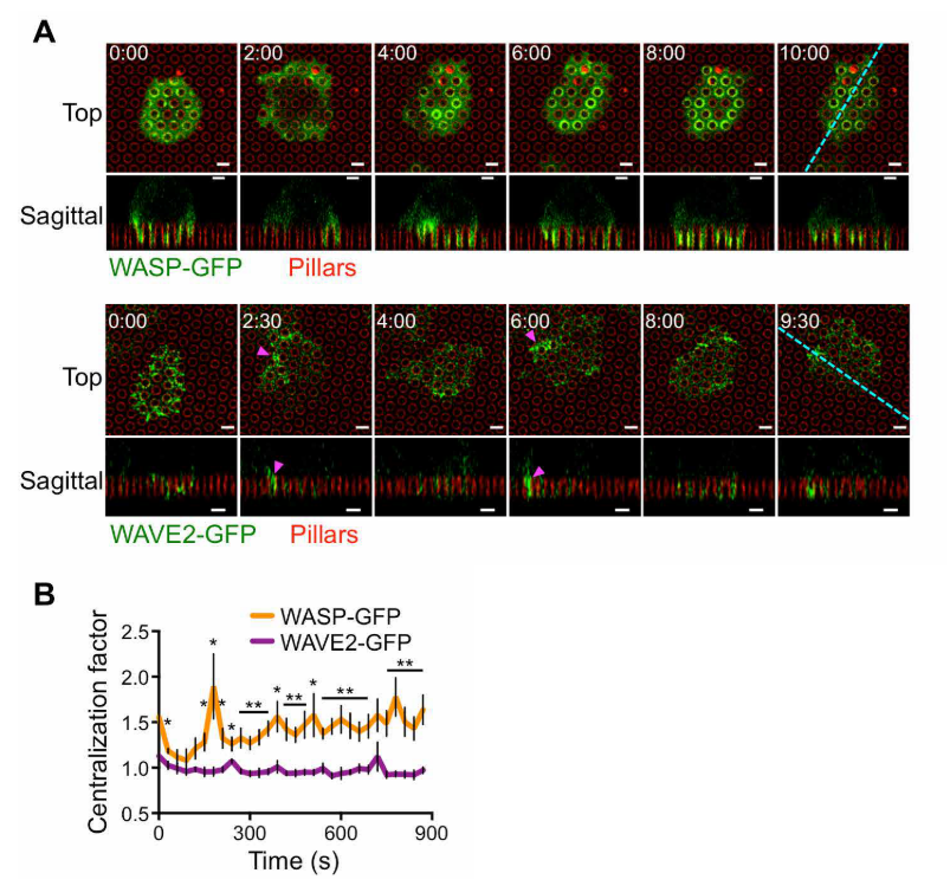
\includegraphics[width=\textwidth]{../figures/chapter2/fig5flprobes.png}
	\caption{WASP and WAVE2 segregate at the synapse.}
	\caption*{\textbf{(A and B)}: OT1 CTLs expressing WASP-GFP or WAVE2-GFP were imaged by confocal microscopy on fluorescent micropillars bearing H2-$K^{b}$-OVA and ICAM1. \textbf{(A)}: Time-lapse montages of representative CTLs, with micropillars shown in red. z-projection images (top views) are shown above with sagittal views below. Cyan dashed lines denote the slicing planes used for the sagittal images. Magenta arrowheads indicate representative lateral accumulations of WAVE2-GFP. \textbf{(B)}: Centralization factor analysis of WASP-GFP and WAVE2-GFP, with time 0 denoting initial contact with the pillars. n = 6 for each cell type. In graphs, *P \textless 0.05 and **P \textless 0.01, calculated by two-tailed Student’s t test comparing WASP-GFP to WAVE2-GFP \textbf{(B)}. Error bars denote SEM. Mitchell Wang, Fella Tamzalit, and Morgan Huse performed these experiments.}
	\label{fig:fig5flprobes}
\end{figure}

To assess the importance of WASP and WAVE2 for IS re-modeling, we used CRISPR (CR)-Cas9 to target the Was and Wasf2 genes, respectively, in OT1 CTLs (Figure \ref{fig:fig5flcrisprs}). WASP- or WAVE2-deficient CTLs prepared in this manner (WASP-CR and WAVE2-CR, respectively) were transduced with Lifeact-GFP and then imaged on micropillar arrays. Whereas control CTLs expressing nontargeting guide RNA (NT-CR) formed protrusions in both the center and the periphery of the IS, the protrusive activity of WASP-CR cells was largely constrained to the periphery (Figure \ref{fig:fig5flcrisprs}a and b). Centralization factor analysis revealed that the F-actin distributions of WAVE2-CR CTLs were more centralized than those of NT-CR controls, which were in turn more centralized than those of WASP-CR CTLs (Figure \ref{fig:fig5flcrisprs}a and b). Hence, WASP deficiency leads to a specific loss of central protrusions, whereas WAVE2 deficiency eliminates peripheral structures. Collectively, these data indicate that WAVE2 controls peripheral F-actin growth involved in lateral motion, whereas WASP drives protrusion formation closer to the center of the IS.

\clearpage
\begin{figure}[htbp]
	\caption{WASP and WAVE2 control distinct subsets of protrusions.}
	\caption*{\textbf{(A}: Time-lapse montages of representative CTLs, with micropillars shown in red. z-projection images (top views) are shown above with sagittal views below. Cyan dashed lines denote the slicing planes used for the sagittal images. \textbf{(B)}: Centralization factor analysis of Lifeact-GFP in NT-CR, WASP-CR, and WAVE2-CR OT1 CTLs, with time 0 denoting initial contact with the pillars. n = 6 for each cell type. In all montages, time in minutes:seconds is indicated in the upper left corner of each top-view image. Scale bars, 2 $\mu$m. In graphs, *P \textless 0.05 and **P \textless 0.01, calculated by two-tailed Student’s t test  WASP-CR (red) and WAVE2-CR (green) to NT-CR \textbf{(B)}. Error bars denote SEM. Mitchell Wang, Fella Tamzalit, and Morgan Huse performed these experiments.}
	\label{fig:fig5flcrisprs}
\end{figure}
\clearpage
\begin{figure}[h!]
	\ContinuedFloat
	\centering
	\captionsetup{labelformat=adja-page}
	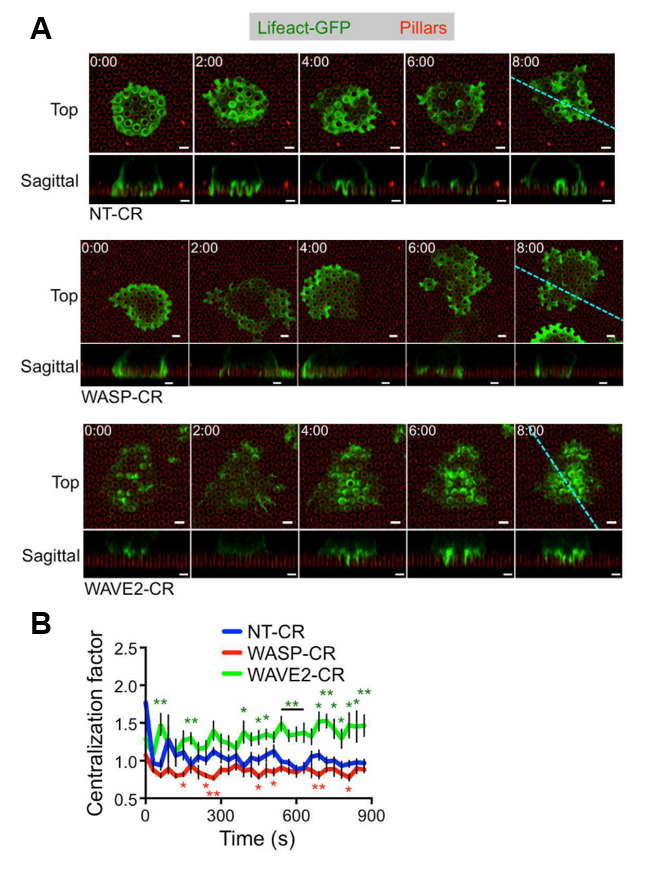
\includegraphics[width=\textwidth]{../figures/chapter2/fig5flcrisprs.png}
	\caption[]{}
\end{figure}

\subsection{WASP and WAVE2 depletion induce distinct functional phenotypes}
Next, we investigated the mechanical consequences of WASP and WAVE2 depletion by imaging NT-CR, WASP-CR, and WAVE2-CR CTLs on narrow micropillar arrays (Figure \ref{fig:fig1pillarscartoon}). WASP-CR CTLs avidly engaged the arrays and deformed them as quickly as did NT-CR controls. The overall magnitude of WASP-CR force exertion, however, was significantly reduced (Figure \ref{fig:fig6pillars}b). By contrast, depletion of WAVE2 delayed the onset of force exertion but did not affect its overall magnitude (Figure \ref{fig:fig6pillars}b). To assess the spatial patterns of these mechanical responses, we plotted the number of strongly deflected pillars as a function of radial distance from the IS COG (Figure \ref{fig:fig6supp}b). NT-CR and WAVE2-CR CTLs induced pillar deflections in both the central IS (\textless 3 $\mu$m from the COG) and the periphery (\textgreater 3 $\mu$m from the COG). By contrast, in WASP-CR CTLs, there was a marked absence of centrally localized events (Figure \ref{fig:fig6crisprs}a). Hence, the capacity to generate protrusions in the center of the IS was associated with force exertion in that domain. 

\begin{figure}[htbp]
	\centering
	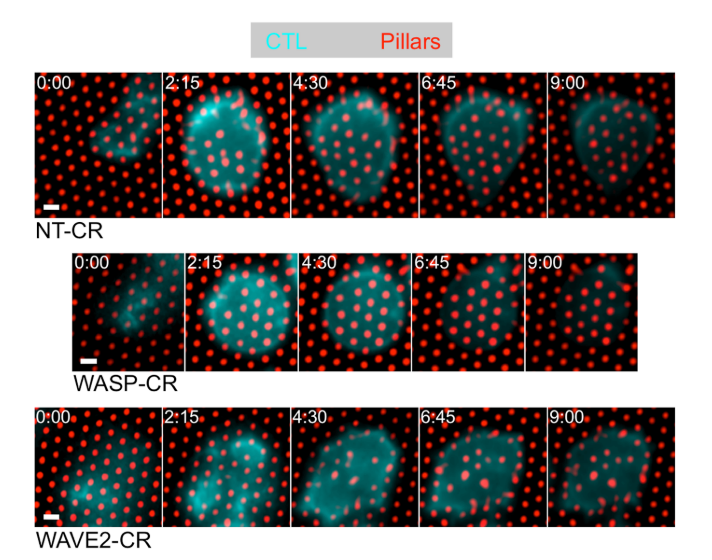
\includegraphics[width=\textwidth]{../figures/chapter2/fig6pillars.png}
	\caption{WASP and WAVE2 depletion induces spatially different patterns of force exertion.}
	\caption*{\textbf{(A and B)}: NT-CR, WASP-CR, and WAVE2-CR OT1 CTLs were labeled with a fluorescent anti-CD45 Fab and imaged on narrow fluorescent micropillars coated with H2-$K^{b}$-OVA and ICAM1. \textbf{(A)}: Time-lapse montages of representative CTLs showing pillar deflection. Time in minutes:seconds is indicated in the upper left corner of each top-view image. Scale bars, 2 $\mu$m. \textbf{(B)}: Total force exertion against pillar arrays was graphed versus time. Color bar above each graph indicates the P value for each time point (two-tailed Student’s t test). Mitchell Wang, Fella Tamzalit, Weiyang Jin, and Morgan Huse performed these experiments.}
	\label{fig:fig6pillars}
\end{figure}

Last, we examined the cytotoxic function of CTLs lacking WASP and WAVE2. WASP depletion induced a significant defect in killing,which we observed using both lymphocytic (RMA-s lymphoma) and adherent (MB49 urothelial carcinoma, B16 melanoma) target cells (Figure \ref{fig:fig6crisprs}b). This defect was most pronounced (around a 50\% reduction) at low levels of antigen. At higher antigen concentrations, however, killing by NT-CR and WASP-CR CTLs was quite comparable. WASP-CR CTLs did not exhibit lower levels of lytic granule fusion (Figure \ref{fig:fig6crisprs}c), indicating that their reduced cytotoxicity could not be attributed to a defect in perforin and granzyme release. Depletion of WAVE2 led to a distinct and somewhat variable cytotoxicity phenotype. In some experiments, we found little to no change in killing and granule fusion, whereas in others, we observed modest reductions that were most pronounced at high antigen concentrations (Figure \ref{fig:fig6crisprs}b, c, \ref{fig:fig6supp}c, d). WAVE2-CR CTLs, but not their WASP-CR counterparts, exhibited significantly reduced conjugate formation (Figure \ref{fig:fig6crisprs}d), implying that WAVE2 promotes target cell adhesion. Consistent with this interpretation, depletion of WAVE2, but not WASP, impaired CTL adhesion to ICAM1-coated surfaces, both in the presence and in the absence of H2-$K^{b}$-OVA (Figure \ref{fig:fig6supp}e). We also examined indices of TCR signaling and found that WASP-CR and WAVE2-CR CTLs exhibited normal TCR-induced $Ca^{2+}$ flux and activation of the MAPK, PI3K, and NF-$\kappa$B pathways (Figure \ref{fig:fig6supp}f and g). Hence, depletion of WASP or WAVE2 does not broadly disrupt early T cell activation. 

\begin{figure}[htbp]
	\centering
	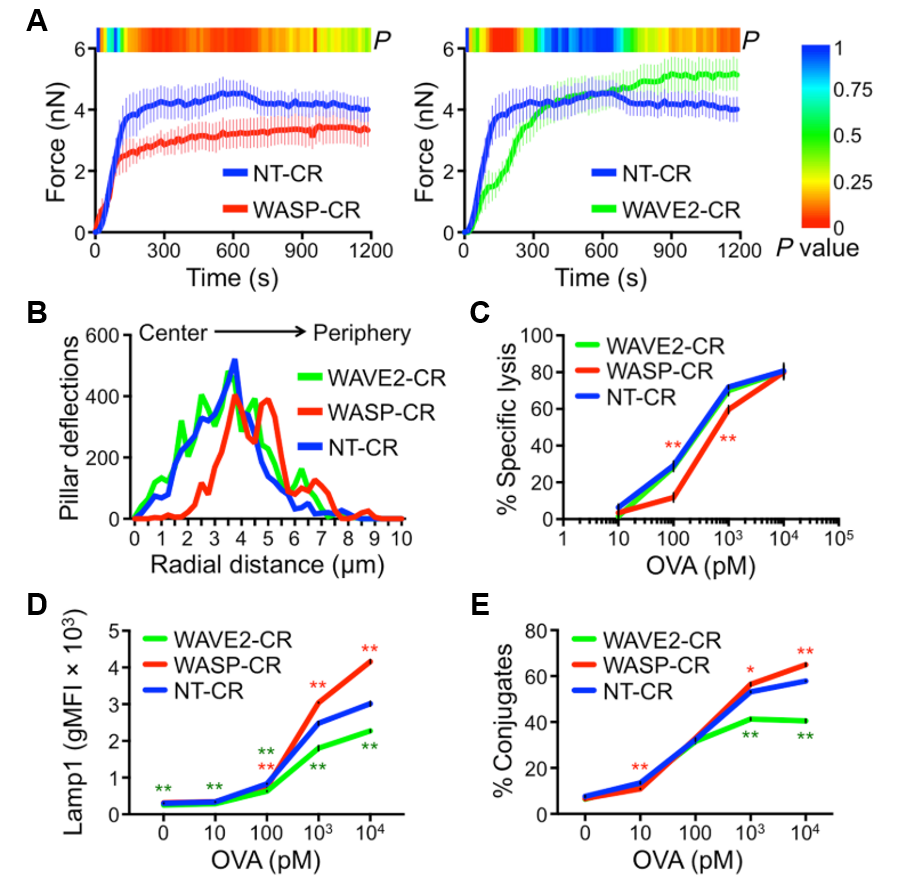
\includegraphics[width=\textwidth]{../figures/chapter2/fig6crisprs.png}
	\caption{WASP and WAVE2 depletion induce distinct cytotoxic phenotypes.}
	\caption*{\textbf{(A)}: Histogram showing the distribution of strong deflections as a function of radial distance from the center of the IS. n = 10 for each cell type in Figure \ref{fig:fig6pillars}. \textbf{(A to D)}: RMA-s target cells were loaded with in- creasing concentrations of OVA and mixed with NT-CR, WASP-CR, or WAVE2-CR OT1 CTLs. \textbf{(B)}: Specific lysis of RMA-s cells. \textbf{(C)}: Lytic granule fusion measured by surface exposure of Lamp1. \textbf{(D)}: CTL–target cell conjugate formation measured by flow cytometry. All error bars denote SEM. In \textbf{(A to D)}, *P \textless 0.05 and **P \textless 0.01, calculated by two-tailed Student’s t test comparing WASP-CR (red) and WAVE2-CR (green) to NT-CR. Mitchell Wang and Fella Tamzalit performed these experiments.}
	\label{fig:fig6crisprs}
\end{figure}

We conclude that WASP plays a more important role than WAVE2 in boosting cytotoxicity and that it does so in a manner independent of TCR signaling, conjugate formation, and granule release. The WASP-CR killing defect was strongest at low antigen concentrations, when granule release was lower and perforin levels were limiting, and it disappeared at high antigen concentrations, when perforin was abundant. Previous studies of CTLs derived from patients with WAS revealed a similar cytotoxicity phenotype: reduced killing (despite normal conjugate formation and granule release), which was rescued by strong TCR stimulation \cite{Calvez2011, DeMeester2010}. This is precisely the pattern of results one would expect after blocking a mechanical process that boosts the per-molecule efficiency of perforin. Together with the imaging data described above, these results suggest a model in which centralized, WASP-dependent protrusions enhance target cell killing through cytolytic mechanopotentiation.

\clearpage
\begin{figure}[htbp]
	\caption{WASP and WAVE2 depletion induce distinct functional phenotypes.}
    \caption*{\textbf{(A)}: Immunoblot analysis of WASP and WAVE2 expression in NT-CR, WASP-CR, and WAVE2-CR CTLs. Actin served as a loading control. Bars denote intensity of WASP and WAVE2 bands. \textbf{(B)}: Diagram schematizing the radial distance histogram analysis of pillar deflections shown in Figure \ref{fig:fig6pillars}. \textbf{(C)}: Adherent MB49 (left) or B16 (right) cells were loaded with increasing concentrations of OVA and then mixed with NT-CR or WASP-CR OT1 CTLs. Target cell lysis was measured by LDH release. \textbf{(D)}: RMA-s target cells were loaded with increasing concentrations of OVA and then mixed with NT-CR, WASP-CR, or WAVE2-CR OT1 CTLs. Specific lysis of RMA-s cells is shown. This experiment highlights the reduced cytotoxicity occasionally observed in WAVE2-CR CTLs at high antigen concentrations. \textbf{(E)}: Adhesion of fluorescently labeled NT-CR, WASP-CR, and WAVE2-CR OT1 CTLs to wells coated with the indicated concentrations of ICAM1 in the absence (top) or presence (bottom) of H2-$K^{b}$-OVA (pMHC). \textbf{(F)}: NT-CR, WASP-CR, and WAVE2-CR OT1 CTLs were loaded with Fura2-AM $Ca^{2+}$ dye and then imaged on stimulatory glass surfaces coated with H2-$K^{b}$-OVA and ICAM1. $Ca^{2+}$ signaling was analyzed by quantifying mean normalized Fura2 ratio over time. N $\geq$ 29 for each cell type. In \textbf{(C-F)}, * and ** indicate P \textless 0.05 and P \textless 0.01, respectively, calculated by two-tailed Student’s T-test comparing WASP-CR (red) and WAVE2-CR (green) to NT-CR. \textbf{(G)}: NT-CR, WASP-CR, and WAVE2-CR OT1 CTLs were stimulated with beads coated with H2-$K^{b}$-OVA and ICAM1 for the indicated times and then lysed. pErk1/2, pAKT, and I$\kappa$B levels were assessed by immunoblot using actin as a loading control. All error bars denote SEM. Mitchell Wang, Fella Tamzalit, and Morgan Huse performed these experiments.}
    \label{fig:fig6supp}
\end{figure}
\clearpage
\begin{figure}[h!]
	\ContinuedFloat
    \centering
    \captionsetup{labelformat=adja-page}
    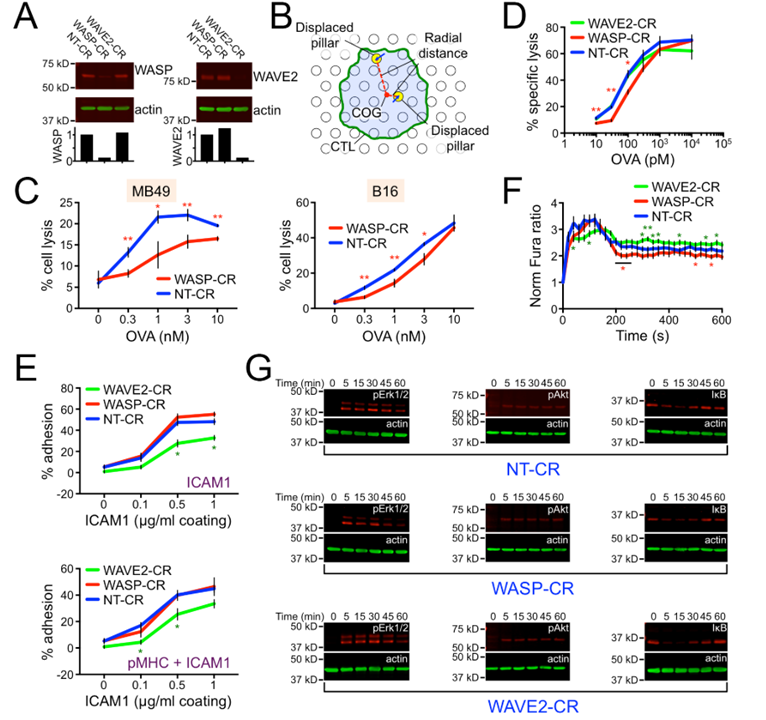
\includegraphics[width=\textwidth]{../figures/chapter2/fig6supp.png}
    \caption[]{}
\end{figure}

\subsection{WASP controls target cell deformation at the IS}
If synaptic protrusions mechanopotentiate perforin function, then they should be capable of physically deforming the target cell surface. To investigate this hypothesis, we performed live imaging experiments using H2-$K^{b}$ murine endothelial cells as targets for OT1 CTLs \cite{Sage2012, Kumari2015}. In culture, endothelial cells adopt a flat, stellate architecture that is stable over time.Hence, deviations in this morphology within the IS can be attributed to the physical activity of the T cell (Figure \ref{fig:fig7lls}a). To facilitate imaging of cellular volume, we prepared endothelial cell lines that expressed mApple or infrared fluorescent protein 670 nm (iRFP670) uniformly in both the cytoplasm and the nucleus. These target cells were loaded with OVA, mixed with OT1 CTLs expressing fluorescently labeled Lifeact, and imaged by lattice light-sheet microscopy. Synapses formed readily and could be identified by their stability, as well as the strong accumulation of interfacial F-actin within the CTL. Within minutes of IS initiation, CTLs generated small, protrusive F-actin structures that invaded the space occupied by the target cell (Figure \ref{fig:fig7lls}b, yellow arrowheads). This was followed shortly thereafter by rapid displacement of the target surface, which was most obvious in conjugates where the CTL attacked from above (Figure \ref{fig:fig7lls}b). This displacement typically occurred before any obvious signs of target cell blebbing, suggesting that it was not part of the apoptotic cascade. CTLs lacking perforin also formed large holes in target cells (Figure \ref{fig:fig7supp}a), further supporting the idea that synaptic deformations result from a physical, rather than a chemical, process. TCR engagement was critical for these mechanical effects. In the absence of antigen, both the speed and the magnitude of target cell displacement diminished substantially (Figure \ref{fig:fig7supp}b), consistent with previous work \cite{Sage2012}. Last, imaging of CTLs expressing Lamp1-GFP revealed that lytic granules accumulated close to areas of deformation (Figure \ref{fig:fig7supp}c), implying that physical manipulation of the target cell contributes to perforin- and granzyme-mediated killing.

\clearpage
\begin{figure}[htbp]
	\caption{WASP controls target cell deformation at the IS.}
    \caption*{\textbf{(A)}: Schematic diagram of a CTL deforming an adherent target cell. (B and C) NT-CR, WASP-CR, and WAVE2-CR OT1 CTLs expressing Lifeact-GFP were applied to cultures of OVA-loaded endothelial target cells expressing iRFP670 and imaged using lattice light-sheet microscopy. \textbf{(B)}: Left: Time-lapse montages of representative “vertically” oriented synapses, with z-projection images (top views) shown above and sagittal views below. Cyan dashed lines denote the slicing planes used for the sagittal images. In z-projection images, target cells are visualized by surface representation. Two z-projections are shown for each time point; Lifeact-GFP is shown on the left and the outline of the CTL of interest is shown on the right. Time in minutes:seconds is indicated in the upper left corner of each sagittal image. Scale bars, 2 $\mu$m. Yellow arrowheads denote protrusive structures in the NT-CR CTL that invade the target cell space. Right: Target IS volume graphed against time, with time 0 denoting IS initiation. Each line corresponds to one CTL–target cell conjugate. \textbf{(C)}: Graph of minimum target IS volume values achieved during the first 400 s of conjugate formation. n = 7 for each cell type. Error bars denote SEM. P value was calculated by two-tailed Student’s t test. Mitchell Wang, Fella Tamzalit, and Morgan Huse performed these experiments.}
    \label{fig:fig7lls}
\end{figure}
\clearpage
\begin{figure}[h!]
	\ContinuedFloat
    \centering
    \captionsetup{labelformat=adja-page}
    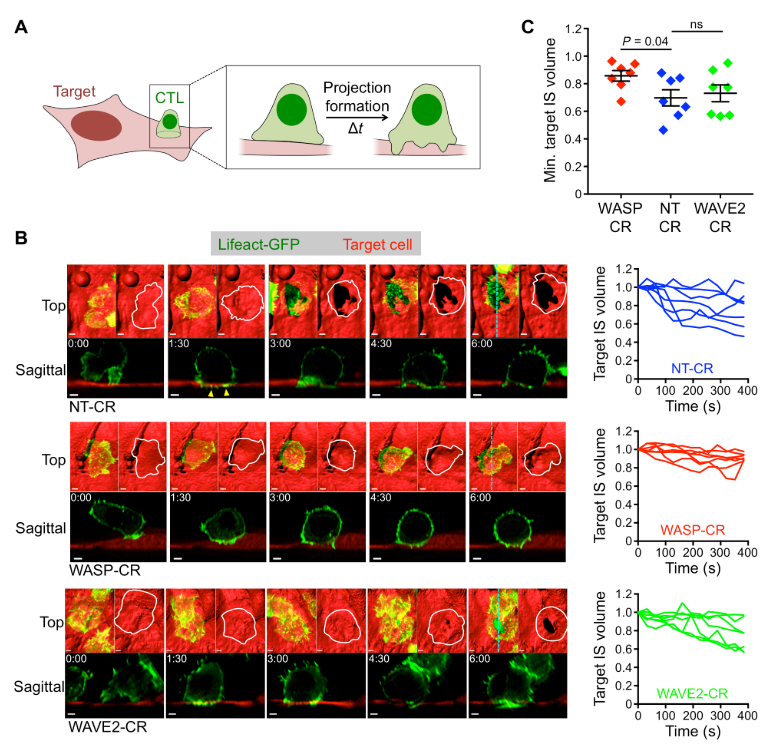
\includegraphics[width=\textwidth]{../figures/chapter2/fig7lls.png}
    \caption[]{}
\end{figure}

Next, we investigated the molecular basis of target cell displacement by comparing synapses formed by NT-CR, WASP-CR, and WAVE2-CR CTLs. Depletion of WASP markedly inhibited physical deformation of the target surface, despite the fact that robust synaptic F-actin accumulation still occurred (Figure \ref{fig:fig7lls}b). To quantify this result, we determined the volume beneath the CTL occupied by the target cell at a given time point and normalized this value to the volume occupied by the target cell in that same region before IS formation (Figure \ref{fig:fig7supp2}). Analysis of this “target IS volume” parameter confirmed that WASP depletion significantly reduced the target cell displacement response (Figure \ref{fig:fig7lls}c). CTLs lacking WAVE2 exhibited a qualitatively distinct phenotype; although they were still capable of substantial deformation, their mechanical responses were somewhat delayed relative to those of NT-CR controls (Figure \ref{fig:fig7lls}b). Collectively, these results mirror the force exertion analysis of WASP-CR and WAVE2-CR CTLs (Figure \ref{fig:fig6pillars}, and they suggest that WASP-dependent synaptic protrusions play a particularly important role in the physical deformation of target cells.

\clearpage
\begin{figure}[htbp]
	\caption{CTLs physically manipulate the target cell surface.}
    \caption*{\textbf{(A-C)}: OT1 CTLs were applied to OVA-loaded endothelial target cells expressing mApple \textbf{(A)} or iRFP670 \textbf{(B and C)} and then imaged using lattice light-sheet microscopy. All time-lapse montages show “vertically” oriented synapses, with z-projection images (top views) shown above and sagittal views below. Target cells are visualized by surface representation in all z- projection images. Cyan dashed lines denote the slicing planes used for the sagittal images. Time in M:SS is indicated in the upper left corner of each sagittal image. Scale bars = 2 $\mu$m. \textbf{(A)} A representative Prf1-/- CTL, visualized using fluorescent Fab fragments against CD45, engaging a target cell. \textbf{(B)}: A representative CTL expressing Lifeact-GFP engaging a target cell in the absence of OVA. In A and B, two z-projections are shown for each time point; the fluorescent signal from the CTL appears on the left and is replaced with an outline of the CTL of interest on the right. \textbf{(C)}: A representative CTL expressing Lifeact-mApple and Lamp1-GFP, engaging a target cell beneath it. The montage above includes the Lifeact-mApple signal, whereas the montage below contains an outline of the CTL of interest. Mitchell Wang, Fella Tamzalit, and Morgan Huse performed these experiments.}
    \label{fig:fig7supp}
\end{figure}
\clearpage
\begin{figure}[h!]
	\ContinuedFloat
    \centering
    \captionsetup{labelformat=adja-page}
    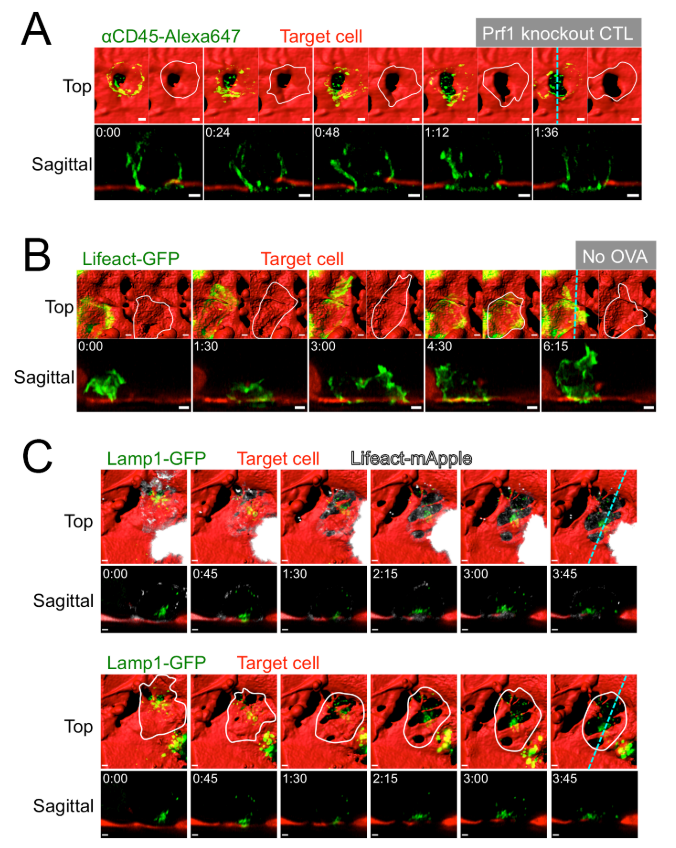
\includegraphics[width=\textwidth]{../figures/chapter2/fig7supp.png}
    \caption[]{}
\end{figure}

\begin{figure}[htbp]
	\centering
	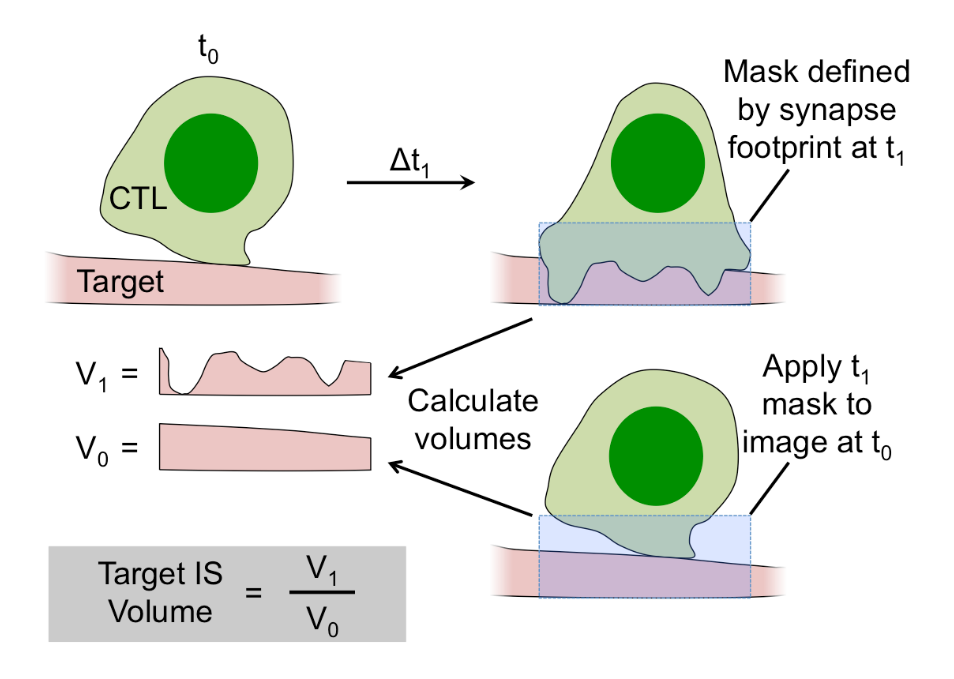
\includegraphics[width=0.9\textwidth]{../figures/chapter2/fig7supp2.png}
	\caption{Target volume analysis.}
	\caption*{Target IS volume compares the endothelial cell volume in the region beneath a CTL at a given time ($V_1$) with the volume occupied by the endothelial cell in that same region at time 0 ($V_0$). Analysis designed by Morgan Huse.}
	\label{fig:fig7supp2}
\end{figure}


\section{Discussion}
The cytotoxic IS boosts perforin toxicity by spatially coordinating its secretion with the exertion of mechanical force. In the present study, we found that perforin release occurs at the base of WASP-dependent, F-actin–rich protrusions (Figure \ref{fig:fig8model}). These protrusions were necessary for synaptic force exertion, particularly in more central regions of the IS close to lytic granules. They were also required for physical deformation of target cells in bona fide cytolytic interactions. WASP-deficient CTLs exhibited a defect in killing that could not be explained by reduced granule release or conjugate formation. Together, these data identify synaptic protrusions as key components of a physical delivery system that enables CTLs to kill target cells with high efficiency. In putting forth this model, we do not suggest that synaptic protrusions are a prerequisite for lytic granule release. Indeed, multiple groups have demonstrated that rigid stimulatory surfaces induce robust cytolytic secretion in the absence of protrusive activity \cite{Beal2009, Rak2011, Ritter2017, Qu2011, Brown2011}. However, the converse relationship may be worth considering, namely, that lytic granule docking and fusion might influence local F-actin architecture and IS mechanics.

\begin{figure}[htbp]
	\centering
	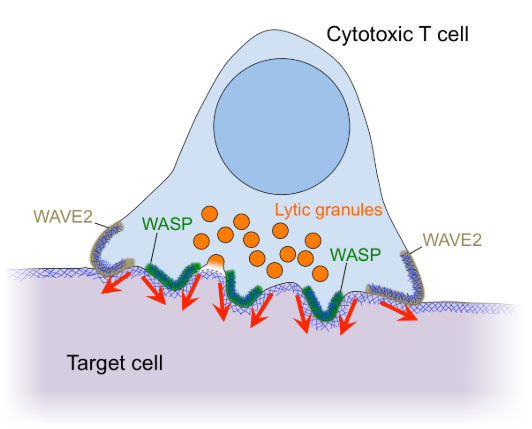
\includegraphics[width=0.8\textwidth]{../figures/chapter2/fig8model.png}
	\caption{Cytolytic mechanopotentiation by WASP-dependent synaptic protrusions.}
	\caption*{Diagram of the cytolytic IS showing peripheral WAVE2-dependent protrusions and central WASP-dependent protrusions. Red arrows denote force exertion.}
	\label{fig:fig8model}
\end{figure}

The marked concentration of granule fusion events at the base of synaptic protrusions implies that mechanisms exist for granule targeting to these domains. Previous studies have highlighted the importance of F-actin clearance for enabling granule access to the plasma membrane \cite{Stinchcombe2006, Ritter2015, Rak2011, Brown2011}. This is consistent with our observation that, on micropillar arrays, granule fusion occurs in transient F-actin–free regions at the base of synaptic protrusions. However, the presence of other F-actin hypodense areas in the CTL, which are not targeted by granules, implies that other factors contribute to the process. Lipid second messengers are known to influence exocytosis and membrane trafficking in a variety of cellular contexts (41). Among these, diacylglycerol is an interesting candidate because it tends to accumulate in central synaptic domains that experience F-actin depletion \cite{Chauveau2014, Liu2013, Basu2014}. Granule delivery via microtubules is another possibility \cite{Wiedemann2006, Butler2009}. We observed that a small subset of microtubules extends into synaptic protrusions, and it will be interesting to explore whether and how this subset contributes to granule trafficking from the centrosome toward fusion sites in the synaptic membrane. Last, it is possible that WASP itself plays a role. A recent super-resolution imaging study demonstrated that WASP promotes granule docking close to regions of integrin clustering \cite{Houmadi2018}. T cells form a variety of protrusive structures at both interfacial and noninterfacial surfaces, which have been documented previously by electron microscopy and high-resolution fluorescence imaging \cite{Sage2012, Cai2017, Carman2007, Ueda2011, Jung2016}. Although the spatial distribution of these protrusions and their dynamics have implied roles in antigen scanning, signaling, and motility, their precise functions have, in most cases, remained undefined. Probably the best-studied are the invadosome-like protrusions (ILPs), which were first observed in T cells initiating diapedesis through endothelial monolayers \cite{Carman2007}. Subsequently, ILPs were also found in antigen-induced synapses formed between T cells and endothelial cells, dendritic cells, or B cells \cite{Sage2012}. ILPs are podosomal structures that are enriched in LFA1 and require WASP and Arp2/3 for their formation \cite{Kumari2015, Carman2007}. The synaptic protrusions we have observed share these characteristics, and it is therefore tempting to speculate that they are a form of ILP. That CTLs might use the same structures to facilitate both diapedesis and target cell killing highlights an underappreciated similarity between the two processes. Both rely on the physical deformation of other cells through direct contact, in the first case to facilitate transmigration and in the second to promote destruction.

The functional defects observed in T cells from patients with WAS and Wasp-/- mice have been attributed to specific effects of WASP on TCR signaling \cite{Kumari2015, Calvez2011, Cannon2004, Dupre2002, Zhang1999}. WASP is expressed by all lymphoid and myeloid lineages \cite{Rivers2017, Massaad2013}, however, and consequently, the phenotypes exhibited by any one immune subset in a WASP-deficient background result not only from the cell-intrinsic functions of the protein but also from the dysfunction of other cell types. Interpreting studies from patient samples is particularly complex because of the wide range of pathological WASP mutations, which vary in their penetrance and can therefore yield markedly distinct disease phenotypes \cite{Massaad2013}. In the present study, we circumvented this complexity by selectively deleting Wasp in CTLs using CRISPR-Cas9 targeting. The resulting cytotoxicity defect was not associated with reduced TCR signaling, $Ca^{2+}$ flux, or granule release, but rather was caused by a failure to generate interfacial protrusions during the effector phase of the response. These data raise the possibility that WASP-dependent protrusions may contribute to interfacial effector pathways in other immune subsets. Previous studies have implicated WASP in macrophage phagocytosis \cite{Leverrier2001, Lorenzi2000}, T cell priming by dendritic cells \cite{Malinova2016, Bouma2011}, and the induction of B cell class switching by follicular T helper cells \cite{Zhang2016}. It will be interesting to investigate how the protrusive activity of WASP influences these and other cell-cell interactions and, in turn, how defects in these interactions contribute to the complex etiology of WAS. In marked contrast to WASP, WAVE2 accumulated in peripheral synaptic protrusions, and CTLs lacking WAVE2 exhibited adhesion and conjugation defects. These observations suggest a role in cell spreading and adhesion that is consistent with previous reports \cite{Nolz2006, Zipfel2006, Nolz2008}. WAVE2 depletion only weakly affected synaptic force exertion and killing, indicating that the protein and the peripheral structures it generates are not involved in cytolytic mechanopotentiation. These results do not exclude the possibility that WAVE2 might promote cytotoxicity in other settings, particularly when target cells are more limiting and robust migration and adhesion are required for their destruction. What is clear from our data, however, is that the functionality of synaptic protrusions is partitioned both spatially (center versus periphery) and molecularly (WASP versus WAVE2). In vitro systems that collapse the IS into two dimensions have been invaluable for investigating its structure and function \cite{Kupfer2010, Balagopalan2011}. The inherent constraints of these systems, however, have limited our understanding in significant ways. It was only by analyzing the IS in an oriented, three-dimensional environment that we were able to assess the formation of synaptic protrusions and to study the implications of these structures for IS mechanics and effector responses. Micropatterned reconstitution systems can reveal unexplored aspects of cellular architecture, and we anticipate that they will become increasingly important in future studies of complex immune cell biology.

\section{Materials and Methods}

\subsection{Study design}
The goal of this study was to understand how CTLs combine cytolytic secretion with force exertion at the IS. We used fluorescence imaging of mouse CTLs, single-cell biophysical assays, and functional experiments. Micropatterned PDMS substrates were used both to visualize the growth of synaptic protrusions and to measure mechanical activity. To perturb protrusion formation and synaptic F-actin dynamics, we used CRISPR-Cas9 technology, shRNA, and the Arp2/3 inhibitor CK666. Experimental sample sizes were not pre-determined, and there were no predefined study end points. Experiments were not randomized, and investigators were not blinded during acquisition and data analysis. In general, experiments were performed at least twice (two biological replicates). Specific information about analysis methods can be found in the “Image analysis” section below.

\subsection{Micropillar preparation}
PDMS (Sylgard 184; Dow Corning) micropillar arrays were prepared as previously described \cite{Bashour2014}. Two types of pillars were used for this study: (i) 1 $\mu$m in diameter, 5 $\mu$m in height, and spaced hexagonally with a 2 $\mu$m center-to-center distance; and (ii) 0.7 $\mu$m in diameter, 6 $\mu$m in height, and spaced hexagonally with a 2-$\mu$m center-to-center distance. Micropillars were cast on chambered coverglass (Lab-Tek), washed with ethanol and phosphate-buffered saline (PBS), and stained with fluorescently labeled streptavidin (20 $\mu$g/ml) (Alexa Fluor 647 or Alexa Fluor 568, Thermo Fisher Scientific) for 2 hours at room temperature. After additional washing in PBS, the arrays were incubated with biotinylated H2-$K^{b}$-OVA and ICAM1 (10 $\mu$g/ml each) overnight at 4\degree C (8). The pillars were then washed into RPMI containing 5\% (v/v) fetal calf serum (FCS) and lacking phenol red for imaging.

\subsection{Live imaging on micropillars}
For force measurements, T cells were stained with Alexa Fluor 488– labeled anti-CD45.2 Fab (clone 104-2) and imaged on fluorescently labeled 0.7-$\mu$m-diameter pillars. Videomicroscopy was performed using an inverted fluorescence microscope (Olympus IX-81) fitted with a 100x objective lens and a mercury lamp for excitation. Images in the 488-nm (CTLs) and 568-nm (pillars) channels were collected every 15 s using MetaMorph software. Protrusion formation was imaged on 1-$\mu$m-diameter pillars stained with Alexa Fluor 647–labeled or Alexa Fluor 568–labeled streptavidin. Cells expressing fluorescent probes were added to the arrays and imaged using a confocal laser scanning microscope fitted with a 40x objective lens and 488-nm, 560-nm, and 642-nm lasers (Leica SP5 or Zeiss LSM 880).

\subsection{Lattice light-sheet imaging}
Lattice light-sheet microscopy was performed as previously described using 488-nm, 560-nm, and 642-nm lasers for illumination and a 25x water immersion objective \cite{Chen2014}. Micropillar arrays were cast on 5-mm-diameter coverslips, which were coated with stimulatory proteins as described above and then mounted for imaging. Movies (3- to 20-s time-lapse intervals) were recorded immediately after addition of fluorescently labeled CTLs using two cameras. We collected 488-nm (30–60 mW laser power) and 560-nm (50 mW laser power) images on one camera and 642-nm (50 mW laser power) images on a second camera. For CTL–target cell imaging, CTLs were added to coverslips bearing 90\% confluent monolayers of mApple- or iRFP670-labeled endothelial cells that had been incubated overnight in 2-$\mu$M OVA. Movies (15- to 20-s time-lapse intervals) were recorded immediately after addition of CTLs. We collected 488-nm (50 mW laser power), 560-nm (200 mW laser power), and 642-nm (200 mW laser power) images on one camera. Raw data were deskewed and deconvolved as previously described \cite{Chen2014} using experimentally derived point spread functions. For two camera experiments, image alignment was performed in MATLAB using reference images of fluorescent beads.

\subsection{Image analysis}
Imaging data were analyzed using SlideBook (3i), Imaris (Bitplane), Excel (Microsoft), Prism (GraphPad), and MATLAB (MathWorks). $Ca^{2+}$ responses were quantified by first normalizing the ratiometric Fura2 response of each cell to the last time point before the initial influx of $Ca^{2+}$ and then by aligning and averaging all responses in the dataset based on this initial time point. To quantify F-actin intensity in fixed images (Figure \ref{fig:fig1ptenprotrusions}, we determined the sum intensity of Alexa Fluor 546–labeled phalloidin in the region beneath the pillar tops for each cell after intensity thresholding. For protrusion enrichment, total Lifeact-GFP intensity in the region beneath the pillar tops was divided by the total Lifeact-GFP intensity in a region of identical volume beginning from the first z-section above the pillar tops and extending upward. Force exertion against 0.7 $\mu$m-diameter pillars was calculated after extracting pillar displacements from the imaging data and then converting these displacements into force vectors using custom MATLAB scripts (17, 18). Radial distributions of pillar deflections (Figure \ref{fig:fig6crisprs}) were generated by calculating the distances between strongly deflected pillars (>0.6 $\mu$m deflection) and the IS COG at each time point (Figure \ref{fig:fig6supp}). COG coordinates for the IS were generated from masks derived from the Alexa Fluor 488 (CTL) channel. To calculate the centralization factor (Figure \ref{fig:fig1granulecentralization} and Figure \ref{fig:fig5flprobes}), we first generated a mask encompassing the entire IS (MC) and a mask containing only the features of interest (e.g., lytic granules) (MF) using xy-projection images. Then, the average distance between every pixel in MC and the COG of MC (DC) was determined and subsequently divided by the average distance between every pixel in MF and the COG of MC (DF) (Figure \ref{fig:fig1centralizationfactor}). Granule polarization (Figure \ref{fig:fig1centralizationfactor}) was quantified by determining the vertical distance between the centroid of a mask encompassing the lytic granules and the deepest CTL protrusion, using xz- or yz-projection images. To calculate target IS volume (Figure \ref{fig:fig7lls}), we generated a three-dimensional mask at a time point of interest by tracing the edges of the IS and then propagating the resulting shape downward to encompass the sample lying directly beneath the CTL. The volume of this region occupied by the target cell was then divided by the volume of this same region occupied by the target cell at time 0 (Figure \ref{fig:fig7supp2}).

\subsection{Killing assay, granule fusion assays, and conjugate formation}
RMA-s target cells were labeled with carboxyfluorescein succinimidyl ester (CFSE) or the membrane dye PKH26, loaded with OVA and mixed in a 96-well V-bottomed plate with CellTrace Violet (CTV)–stained OT1 CTLs. To assess killing, we mixed cells at a 1:3 effector: target (E:T) ratio and incubated them for 4 hours at 37 \degree C. Specific lysis of CFSE+ target cells was determined by flow cytometry \cite{Purbhoo2004}.

For granule fusion assays, the E:T ratio was 1:1, and cells were incubated at 37\degree C for 90 min in the presence of eFluor 660–labeled anti-Lamp1 (clone eBio1D4B; eBioscience). Lamp1 staining was then assessed by flow cytometry. To measure conjugate formation, we mixed CTLs and targets 1:1, lightly centrifuged (100g) the mixture to encourage cell contact, and incubated the mixture for 20 min at 37\degree C. Cells were then resuspended in the presence of 2\% paraformaldehyde, washed in fluorescence- activated cell sorting buffer (PBS + 4\% FCS), and analyzed by flow cytometry. Conjugate formation was quantified as (CFSE+ CTV+)/(CTV+). For killing of adherent target cells, MB49 or B16 cells were cultured overnight on fibronectin and then pulsed with OVA for 2 hours. OT1 CTLs were added at a 4:1 E:T ratio and incubated for 3 hours (MB49 cells) or 4 hours (B16) at 37\degree C in RPMI medium supplemented with interleukin-2 (30 IU/ml). Target cell death was quantified with an LDH (lactate dehydrogenase) cytotoxicity assay kit (Clontech) using the manufacturer’s recommended protocol. All functional assays were performed in triplicate.

\subsection{Statistical analysis}
Figures show representative experiments. Analysis was carried out using either representative experiments or pooled data as indicated (n refers to the number of cells analyzed). Statistical analyses (unpaired or paired t tests) were carried out using GraphPad Prism or Microsoft Excel. All error bars denote SEM.

\subsection{Constructs}
Retroviral expression constructs for Lifeact-GFP, Lifeact-mRuby2, DynPH-GFP, and pHluorin-Lamp1 were previously described \cite{LeFloch2013, Rak2011}. The Lamp1-GFP, WASP- GFP, and WAVE2-GFP constructs were prepared by ligating the full-length coding sequences of mouse Lamp1, mouse WASP, and human WAVE2 into a pMSCV retroviral expression vector upstream of GFP \cite{Purbhoo2004}. The Lifeact-mApple fusion was prepared by PCR from an mApple-N1 template plasmid using oligos that encoded the Lifeact peptide N-terminal to mApple, followed by subcloning into pMSCV. shRNA constructs (shNT and shPTEN) \cite{LeFloch2013} were subcloned into the miR30E vector using the following primers: miRE-Xho-fw ($5’$-\emph{TGAACTCGAGAAGGTATAT TGCTGTTGACAGTGAGCG}-$3’$) and miRE-EcoOligo-rev (5’-TCTCGAATTCT AGCCCCTTGAAGTCCGAGGCAGTAGGC -3’). gRNAs targeting WASP and WAVE2 were generated as previously described using the following oligos: NT gRNA: oligo-1 (5’- CACCGGGATACCTGGGCCGACTTTC -3’) and oligo-2 (5’- AAACGAAAGTCGGCCCAGGTATCCC -3’). WASP gRNA: oligo-1 (5’- CACCGCTGGACCATGGAACACTGCG -3’) and oligo-2 (5’-
AAACCGCAGTGTTCCATGGTCCAGC -3’). WAVE2 gRNA: oligo-1 (5’-CACCGAGCAAGGGAGTTTACTCGGG-3’) and oligo-2 (AAACCCCGAGTAAACTCCCTTGCTC -3’). Each gRNA was cloned into the LentiGuide-Puro vector and then amplified by PCR using the following primers: LMP BamHI F2 (5’- TTTTTGGATCCTAGTAGGAGGCTTGGTAG -3’) and LMP EcoRI R2 (5’- TTTTTGAATTCTGTCTACTATTCTTTCCC -3’). The resulting fragments were digested with BamHI and EcoRI and ligated into miR30E previously digested with EcoRI and BglII.

\subsection{Cells and small molecule inhibitors}
The animal protocols used for this study were approved by the Institutional Animal Care and Use Committee of Memorial Sloan- Kettering Cancer Center. Primary CTL blasts were prepared by pulsing irradiated C57BL/6 splenocytes with 100 nM OVA and then mixing them with T cells from OT1 $\alpha$ $\beta$ TCR transgenic mice in RPMI medium containing 10\%(vol/vol) FCS. Cells were supplemented with 30 IU/ml IL2 after 24 h and were split as needed in RPMI medium containing 10\% (vol/vol) FCS and IL2. RMA-s cells were maintained in RPMI containing 10\% (vol/vol) FCS, while C57BL/6 murine cardiac microvascular endothelial cells (CellBiologics), MB49 cells, and B16 cells were maintained in DMEM medium containing 10\% (vol/vol) FCS. To inhibit Arp2/3, CTLs were preincubated with CK666 (100-150 µM, Sigma-Aldrich) for 10 min at 37\degree C, and CK666 was then maintained at the same concentration for the duration of the experiment.

\subsection{Retroviral transduction}
Phoenix E cells were transfected with expression vectors and packaging plasmids using the calcium phosphate method. Ecotropic viral supernatants were collected after 48 h at 37\degree C and added to 1.5 × $10^{6}$ OT1 blasts 2 days after primary peptide stimulation. Mixtures were centrifuged at 1400 × g in the presence of polybrene (4 $\mu$g/ml) at 35\degree C, after which the cells were split 1:3 in RPMI medium containing 10\% (vol/vol) FCS and 30 IU/ml IL2 and allowed to grow for an additional 4-6 days.

\subsection{Fixed imaging}
OT1 cells were incubated on stimulatory micropillars for 20 min at 37\degree C, fixed by adding 4\% paraformaldehyde for 5 min, and washed with PBS. Samples were then blocked in PBS solution supplemented with 2\% goat serum for 1 h at room temperature and stained overnight at 4\degree C with anti-$\beta$-tubulin (clone TUB 2.1; Sigma) or anti-LFA1 (clone M17/4; eBioscience). Actin was visualized using Alexa 546-labeled phalloidin (ThermoFisher Scientific). After washing, samples were incubated with the appropriate secondary antibody for 2 h at room temperature, washed and imaged using a Leica SP8 confocal laser scanning microscope fitted with a white light laser and a 40x objective lens.

\subsection{$Ca^{2+}$ imaging}
CTLs were loaded with 5 $\mu$g/ml Fura2-AM (ThermoFisher Scientific), washed, and then imaged on stimulatory glass surfaces coated with H2-$K^{b}$-OVA and ICAM-1 as previously described. Images were acquired using 340 nm and 380 nm excitation every 30 seconds for 30 min with a 20x objective lens (Olympus).

\subsection{Adhesion assay}
Integrin-mediated adhesion was measured in flat-bottomed 96-well plates bearing increasing densities of ICAM1. The plates were coated with 10 $\mu$g/ml streptavidin in PBS followed by increasing concentrations of biotinylated ICAM1 in the presence or absence of 1 $\mu$g/ml biotinylated H2-$K^{b}$-OVA in Hepes buffered saline (10 mM Hepes pH 7.5, 150 mM NaCl) with 2 \% BSA. The total concentration of biotinylated protein during coating was kept at 5 $\mu$g/ml by the addition of nonspecific biotinylated MHC (H2-$D^{b}$). OT1 CTLs were fluorescently labeled with cell trace violet (CTV), resuspended in adhesion buffer (PBS with 0.5\% BSA, 2 mM $MgCl_2$, 1 mM $CaCl_2$), and added to ICAM1-bearing wells in triplicate. After a 20 min incubation at 37\degree C, wells were washed with warmed adhesion buffer as described, and the bound cells quantified by fluorimetry.

\subsection{Immunoblot}
0.2-1 x $10^{6}$ CTLs were lysed using cold cell lysis buffer containing 50 mM TrisHCl, 0.15 M NaCl, 1 mM EDTA, 1\% NP-40 and 0.25\% sodium deoxycholate. Suppression of PTEN, WASP, and WAVE2 was confirmed using the following antibodies: anti-PTEN monoclonal antibody (clone D4.3; Cell Signaling Technology), anti-WASP monoclonal antibody (clone B-9; Santa Cruz) and anti-WAVE2 monoclonal antibody (clone D2C8; Cell Signaling Technology). Actin served as a loading control (clone AC-15, Sigma). For signaling assays, serum and IL2 starved OT1 CTLs were incubated with streptavidin polystyrene beads (Spherotech) coated with H2-$K^{b}$-OVA and ICAM1 at a 1:1 ratio for various times at 37\degree C and immediately lysed in 2 × cold lysis buffer containing phosphatase inhibitors (1 mM NaF and 0.1 mM Na3VO4) and protease inhibitors (cOmplete mini cocktail, EDTA-free, Roche). Activation of PI3K, MAP kinase and NF-$\kappa$B signaling was assessed by immunoblot for pAkt (Phospho-Akt (Ser473) Ab; Cell Signaling Technology), pErk1/2 (Phospho-Thr202/ Tyr204; clone D13.14.4E; Cell Signaling Technology), and I$\kappa$B (Cell Signaling Technology).
